\documentclass[12pt]{article}

\usepackage{graphicx}
\usepackage{caption}
\usepackage{subcaption}
\usepackage[spanish]{babel}
\usepackage[utf8]{inputenx}
\usepackage{anysize} 
\usepackage{amsmath}
\usepackage{listings}
%\usepackage{wrapfig} % paquete gráfico... quizás es necesario actualizar paquetes en kile
\usepackage{hyperref}

\usepackage{fancyhdr}
\pagestyle{fancy}

\hypersetup{
    colorlinks,%
    citecolor=black,%
    filecolor=black,%
    linkcolor=black,%
    urlcolor=black
}
\marginsize{1cm}{1cm}{1cm}{1cm} %izq der arriva abajo

\title{Informe preliminar}
\author{Facundo Nahuel Uriel Silva}

\lhead{ \chaptername }

 
\begin{document}

  %Caratula
  \newpage
  \thispagestyle{empty}
  
  \begin{center}
    
\includegraphics[width=250px]{../../logo_fiuba_alta.jpg} 

  \vspace{100px}

  {\bf \Huge{Trabajo Profesional de Ingeniería Electrónica} }
  
  \vspace{50px}

  \huge{ Sistema de control para proceso de sinterizado de nano estructuras }

  \vspace{50px}

  \huge{ \textit{Requerimientos técnicos del cliente} } 

  \end{center}

  \vspace{70px}

   \begin{bf}
    \begin{Large}
      \begin{tabbing}
	\= ----- \= ----- \= --------------------- \= \kill
	\> Integrantes:\\
	\\
	  \>\> Estanislao López Morgan \\
	  \>\>\>  Padrón:	\> 84546 \\
	  \>\>\>  Mail:	\>\url{estanux@gmail.com} \\
	\\
	  \>\> Facundo Nahuel Uriel Silva\\
	  \>\>\>  Padrón:	\> 86881 \\
	  \>\>\>  Mail:	\> \url{fanaur@gmail.com}\\
      \end{tabbing}
    \end{Large}
  \end{bf}



  %Indice de contenidos
  \newpage
  
  
  \thispagestyle{empty} \tableofcontents \thispagestyle{empty} %asi se se hace el número de pagina

  %Comienzo
 
  
  %\section{Introducción}
   %\newpage
 \newpage
\setcounter{page}{1}

\section{Requisitos Técnicos}

\subsection{Preguntas}
  
 \begin{enumerate} 
      \item \textbf{ Proceso de sinterizado }
	\begin{enumerate}
	  \item ¿Que magnitudes físicas se deben medir?
	  \item ¿Cual es el mínima corriente requerida para el proceso?
	  \item ¿Cual es el máxima corriente de pico esperada?
	  \item ¿Cual es el orden de magnitud de la impedancia eléctrica de la muestra de polvos?
	  \item ¿Se experimentará con distintos tipos de polvos?
          \item ¿Qué materiales en particular se van utilizar como muestra a sinterizar?
          \item ¿Se proyecta que a futuro se utilice otros materiales?¿Cómo afectaría esto al proceso?
          \item ¿Existe algún proceso por el cual se puede determinar que la muestra está sinteizada correctamente?¿Se desea implementar?
	  \item ¿Existirá un único banco de capacitores (descargar múltiples secuenciales)?
	  \item ¿Con qué periodicidad se estima realizar el proceso (horas, días, semanas)?
	  \item ¿En cuanto a la compresión mecánica, qué prensa se utilizará?
	  \item ¿El valor de presión que se establece antes de empezar la descarga, debe reajustarse durante el proceso?¿Cual tiene que ser este valor constante?

	\end{enumerate}
	  
      \item \textbf{ Interfaz de usuario }
	\begin{enumerate}
	  \item ¿Cómo se desea visualizar los datos obtenidos del proceso?
	  \item ¿Es necesario un que el sistema tenga un display ?¿ Y teclado?
	  \item ¿Se necesita accionar en forma manual algún parámetro del proceso, Cuál?
	  \item ¿En necesario visualizar los datos en forma remota (vía Web)?
	  \item ¿Se cuenta con bocas de red cerca de la zona de emplazamiento del dispositivo?¿Se planea hacerlo?	  
	  \item Los datos de la experimentación, ¿Deben quedar guardados en el dispositivo o un servidor local?
	  \item ¿Es necesario tener la posibilidad de guardar los datos en un pendrive?	  
	  \item ¿Se desea genera alguna extensión de archivo en particular?
	  \item ¿Cómo desea configurar el sistema de control?
	  \item ¿Que parámetros del proceso se deben visualizar y cuales almacenar (magnitudes física)?
	  \item ¿Qué parámetros de control tiene el proceso (condiciones que se deben cumplir para iniciar el proceso. Ejemplo: nivel de carga)?
	  \item ¿Qué parámetros de control deberían ser establecidos de forma remota y cuales de forma local?
	  \item ¿Se necesita accionar en forma manual algún parámetro del proceso?¿Cuál?
	\end{enumerate}
      
      \item \textbf{ Seguridad }
	\begin{enumerate}
	  \item ¿Es necesario algún parámetro de seguridad en especial?¿Qué es lo más crítico del proceso?
	  \item ¿El operario estará en el mismo ambiente de la experimentación?
	  \item ¿Debe haber elementos contra incendios?
	  \item ¿Es necesario un nivel de autorización para operar el dispositivo (login)?
	\end{enumerate}
      
    \end{enumerate}

\newpage

\section{Diagrama en bloque de la solución propuesta}

\begin{figure}[h!]
 \centering
 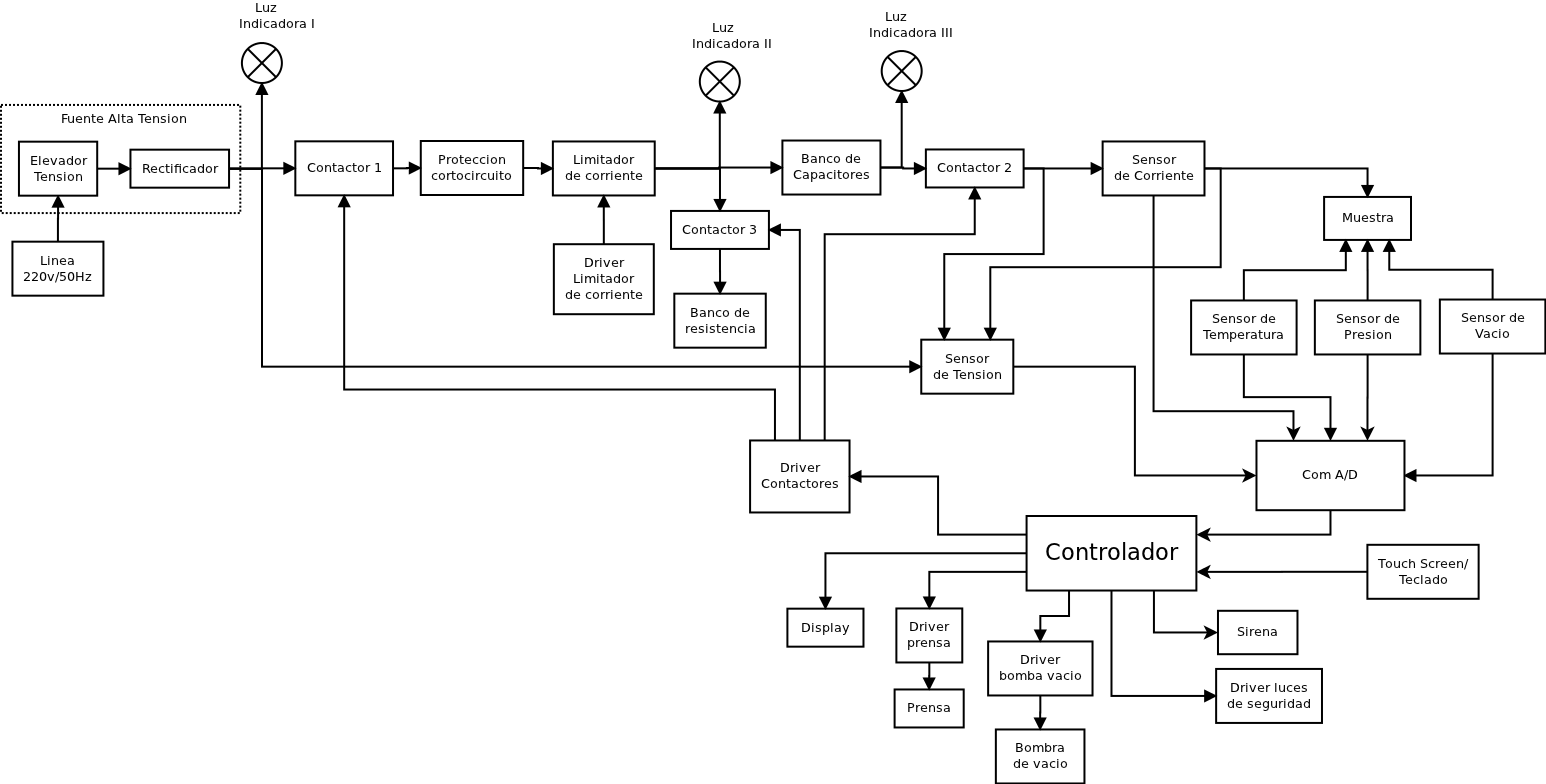
\includegraphics[height=330px, angle=90]{../../Diagramas/diagramaBloquesMacro.png}
 \caption{Diagrama en bloques general de la solución propuesta}
\end{figure}


  %Bibliografia
 % \newpage

  %\begin{thebibliography}{1}
  %  \bibitem{ ECAS_tecnologys_page } \url{ http://iopscience.iop.org/1468-6996/10/5/053001 }
  %  \bibitem{ ECAS_tecnologys_pdf } \url{ http://iopscience.iop.org/1468-6996/10/5/053001/pdf/1468-6996_10_5_053001.pdf }
  %  \bibitem{ ECAS_wiki } \url{ http://en.wikipedia.org/wiki/Capacitor_discharge_sintering }    
  %  \bibitem{ Capacitores Leyden } \url{ http://www.leyden.com.ar/esp/index.html }

  %\end{thebibliography}
    

\end{document}